
\documentclass{article}
\usepackage[T1]{fontenc}
\usepackage[utf8]{inputenc}
\usepackage[swedish]{babel}
\usepackage{amsmath, amssymb, mathtools}
\usepackage{enumitem}
\usepackage{siunitx}
\usepackage{listings}
\usepackage{comment}
\usepackage{tikz, pgfplots}
\usepackage{afterpage}
\usepackage{booktabs}

\makeatletter
\def\fps@figure{hbtp}
\def\fps@table{hbtp}
\makeatother

\pgfplotsset{compat=newest}
\sisetup{
	round-mode      = places,
	round-precision = 3
	}

\lstset{
	breaklines=true,
	postbreak=\mbox{\textcolor{red}{$\hookrightarrow$}\space},
	}

\DeclareMathOperator\Poisson{Pois}
\DeclareMathOperator\GammaDist{Gamma}
\DeclareMathOperator\Normal{Normal}
\DeclareMathOperator\Uniform{Uniform}

\title{Third Assignment in MVE550}
\author{Axel Forsman, Jonas Lauri}

\begin{document}
% \maketitle

\section{Question 1}
\begin{enumerate}[label=(\alph*)]
	\item Fin.
\end{enumerate}

\subsection{(a)}
$(N_A)_{A \subseteq \mathbb R^2}$ is a spatial Poisson process
with parameter $\lambda = 36$.
Let $A \coloneqq [0.2, 0.6] \times [0.2, 0.6] \subseteq \mathbb R^2$.
Then $N_A$ has a Poisson distribution with parameter $\lambda \lvert A \rvert$.
Whence we get
$$ \mathbb P(N_A \ge 6) = 1 - \mathbb P(N_A \le 5) = 1 - \Poisson(5; 36 \cdot 0.4^2)
	\approx \num{0.5150434} $$

	\subsection{(b)}
	\begin{center}
		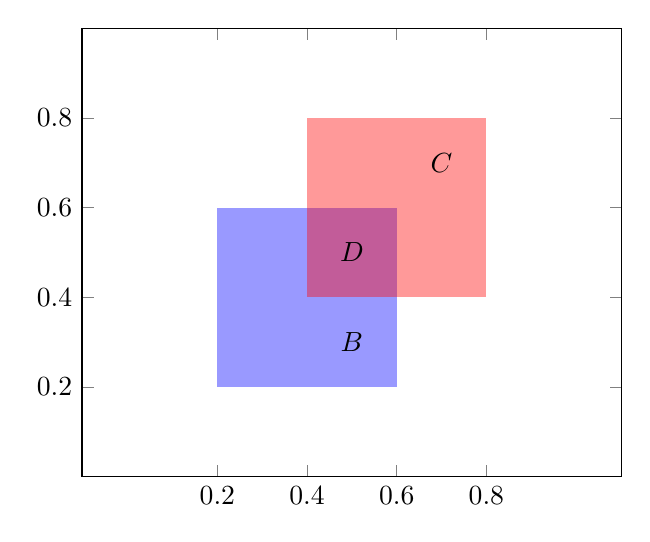
\begin{tikzpicture}
			\begin{axis}[xmin = 0, xmax = 1, ymin=0, ymax = 1, axis equal,
				xtick = {0.2, 0.4, 0.6, 0.8}, ytick = {0.2, 0.4, 0.6, 0.8},
				clip = false]
				\fill[blue, fill opacity=0.4] (0.2, 0.2) rectangle (0.6, 0.6);
				\fill[red, fill opacity=0.4] (0.8, 0.8) rectangle (0.4, 0.4);
				\node at (0.5, 0.3) {$B$};
				\node at (0.7, 0.7) {$C$};
				\node at (0.5, 0.5) {$D$};
			\end{axis}
		\end{tikzpicture}
	\end{center}

\begin{align*}
	\mathbb P(N_{B \cup D = 4}, N_{C \cup D = 4}) &= \sum_{k=0}^4 \mathbb P(N_D = k) \underbrace{\mathbb P(N_{B \cup D} = 4, N_{C \cup D} = 4 \mid N_D = k)}_{\mathbb P(N_B = 4 - k, N_C = 4 - k)} \\
	&= \sum_{k=0}^4 \mathbb P(N_D = k) \mathbb P(N_B = 4 - k) \mathbb P(N_C = 4 - k) \\
	&\approx \num{0.023902}
\end{align*}
where we have used that $N_B, N_C$ are independent since $B, C$ are disjoint.

\begin{comment}
	\appendix
	\section{Appendix, R code}
	\lstinputlisting[language=R]{ass2.R}
\end{comment}

\end{document}
